\documentclass[12pt]{article}
\usepackage[margin=0.75in]{geometry}
\usepackage{float}
\usepackage{multicol}
\usepackage{lmodern}
\usepackage{amssymb,amsmath}
\usepackage{ifxetex,ifluatex}
\usepackage{fixltx2e} % provides \textsubscript
\ifnum 0\ifxetex 1\fi\ifluatex 1\fi=0 % if pdftex
  \usepackage[T1]{fontenc}
  \usepackage[utf8]{inputenc}
\else % if luatex or xelatex
  \ifxetex
    \usepackage{mathspec}
    \usepackage{xltxtra,xunicode}
  \else
    \usepackage{fontspec}
  \fi
  \defaultfontfeatures{Mapping=tex-text,Scale=MatchLowercase}
  \newcommand{\euro}{€}
\fi
% use upquote if available, for straight quotes in verbatim environments
\IfFileExists{upquote.sty}{\usepackage{upquote}}{}
% use microtype if available
\IfFileExists{microtype.sty}{%
\usepackage{microtype}
\UseMicrotypeSet[protrusion]{basicmath} % disable protrusion for tt fonts
}{}
\usepackage{graphicx}
\makeatletter
\def\maxwidth{\ifdim\Gin@nat@width>\linewidth\linewidth\else\Gin@nat@width\fi}
\def\maxheight{\ifdim\Gin@nat@height>\textheight\textheight\else\Gin@nat@height\fi}
\makeatother
% Scale images if necessary, so that they will not overflow the page
% margins by default, and it is still possible to overwrite the defaults
% using explicit options in \includegraphics[width=3.5in][width, height, ...]{}
\setkeys{Gin}{width=\maxwidth,height=\maxheight,keepaspectratio}
\ifxetex
  \usepackage[setpagesize=false, % page size defined by xetex
              unicode=false, % unicode breaks when used with xetex
              xetex]{hyperref}
\else
  \usepackage[unicode=true]{hyperref}
\fi
\hypersetup{breaklinks=true,
            bookmarks=true,
            pdfauthor={Brandon LeBeau},
            pdftitle={PSQF 4143: Section 9},
            colorlinks=true,
            citecolor=blue,
            urlcolor=blue,
            linkcolor=magenta,
            pdfborder={0 0 0}}
\urlstyle{same}  % don't use monospace font for urls
\setlength{\parindent}{0pt}
\setlength{\parskip}{6pt plus 2pt minus 1pt}
\setlength{\emergencystretch}{3em}  % prevent overfull lines
\setcounter{secnumdepth}{0}

\title{PSQF 4143: Section 9}
\author{Brandon LeBeau}
\date{}

\begin{document}
\maketitle

\section{Review}\label{review}

\begin{itemize}
\itemsep1pt\parskip0pt\parsep0pt
\item
  For a randomly selected sample of size \(n\) with a mean \(\mu\) and a
  standard deviation \(\sigma\), the following is true:

  \begin{enumerate}
  \def\labelenumi{\arabic{enumi}.}
  \itemsep1pt\parskip0pt\parsep0pt
  \item
    The distribution of sample means \(\bar{X}\) is approximately
    normal, regardless of the population distribution.
  \item
    The mean of the distribution of sample means is equal to the mean of
    the population distribution, \(\mu_{x} = \mu\).
  \item
    The standard deviation of the distribution of sample means is equal
    to: \(\sigma_{\bar{X}} = \frac{\sigma}{\sqrt{n}}\)
  \end{enumerate}
\end{itemize}

\section{Using the Central Limit
Theorem}\label{using-the-central-limit-theorem}

\begin{itemize}
\itemsep1pt\parskip0pt\parsep0pt
\item
  The average length of time a person stays at a job is 4.4 years with a
  standard deviation (\(\sigma_{X}\)) of 1.8 years.
\item
  With the Normal Distribution: What proportion of employees stay more
  than 7 years on the job?

  \begin{itemize}
  \itemsep1pt\parskip0pt\parsep0pt
  \item
    \(z = \frac{x - \mu}{\sigma} = 1.44, A = .074\)
  \end{itemize}
\item
  With the CLT: What proportion of \emph{sample means} would have values
  greater than 7 years? (i.e.~What proportion of samples of size 10
  would have an average years on the job greater than 7?)

  \begin{itemize}
  \itemsep1pt\parskip0pt\parsep0pt
  \item
    \(z = \frac{\bar{X} - \mu_{\bar{X}}}{\sigma_{\bar{X}}} = \frac{\bar{X} - \mu}{\frac{\sigma}{\sqrt{n}}} = 4.57, A < .0001\)
  \end{itemize}
\end{itemize}

\section{Estimating Population
Parameters}\label{estimating-population-parameters}

\begin{itemize}
\itemsep1pt\parskip0pt\parsep0pt
\item
  The point estimate of the population mean would be the sample mean.

  \begin{itemize}
  \itemsep1pt\parskip0pt\parsep0pt
  \item
    The sample mean would vary from sample to sample.
  \item
    One problem, is that the sample mean does not give us an idea of the
    accuracy to the real value.
  \item
    Our solution is to use a confidence interval.
  \end{itemize}
\end{itemize}

\section{Estimating Population Parameters
2}\label{estimating-population-parameters-2}

\begin{itemize}
\itemsep1pt\parskip0pt\parsep0pt
\item
  The confidence interval is a set of values that tell us with a
  specified accuracy level that the value of the parameter is contained
  within the values.
\end{itemize}

Point Estimate \(\pm\) Critical Value \(*\) Standard Error\\C\% CI of
\(\mu\): \(\bar{X} \pm z_{crit} * \frac{\sigma}{\sqrt{n}}\)\\- Where
\(\pm z\) are the z-scores such that the proportion (or area) of the
curve within the z-scores is equal to the confidence level. -
\(\pm z_{crit} * \frac{\sigma}{\sqrt{n}}\) is referred to as the
\textbf{Margin of Error}.

\section{Alpha}\label{alpha}

\begin{itemize}
\itemsep1pt\parskip0pt\parsep0pt
\item
  Level of confidence refers to the probability that the researcher is
  making a correct conclusion.\\
\item
  There is an amount of error associated with the confidence.
  \textbf{Alpha} is the probability of an incorrect
  conclusion.\\\[ \frac{C\%}{100} = 1 - \alpha \]\\
\item
  We will talk more about this in the next chapter.
\end{itemize}

\section{\texorpdfstring{Confidence Interval for
\(\mu\)}{Confidence Interval for \textbackslash{}mu}}\label{confidence-interval-for-mu}

\begin{itemize}
\itemsep1pt\parskip0pt\parsep0pt
\item
  A 90\% confidence interval for
  \(\mu\):\\\[ \bar{X} \pm 1.64 * \frac{\sigma}{\sqrt{n}} \]
\item
  A 95\% confidence interval for
  \(\mu\):\\\[ \bar{X} \pm 1.96 * \frac{\sigma}{\sqrt{n}} \]
\item
  A 99\% confidence interval for
  \(\mu\):\\\[ \bar{X} \pm 2.58 * \frac{\sigma}{\sqrt{n}} \]
\end{itemize}

\section{Example}\label{example}

\begin{itemize}
\itemsep1pt\parskip0pt\parsep0pt
\item
  A team statistician for the University of Iowa wants to estimate the
  average number of points the team will score during the season. The
  population mean is unknown, but the population standard deviation is 5
  points. A random sample of 12 games was selected from the past two
  seasons; the average number of points scored was 27.4.

  \begin{itemize}
  \itemsep1pt\parskip0pt\parsep0pt
  \item
    What is the best point estimate of the population mean?\\
  \item
    What is the standard error?
  \item
    What is the 95\% confidence interval?
  \item
    What is the 99\% confidence interval?
  \end{itemize}
\end{itemize}

\section{Example 2}\label{example-2}

\begin{itemize}
\itemsep1pt\parskip0pt\parsep0pt
\item
  A team statistician for the University of Iowa wants to estimate the
  average number of points the team will score during the season. The
  population mean is unknown, but the population standard deviation is 5
  points. A random sample of 24 games was selected from the past two
  seasons; the average number of points scored was 27.4.

  \begin{itemize}
  \itemsep1pt\parskip0pt\parsep0pt
  \item
    What is going to change in this example compared to the previous
    example?
  \item
    What is the best point estimate of the population mean?\\
  \item
    What is the standard error?
  \item
    What is the 95\% confidence interval?
  \item
    What is the 99\% confidence interval?
  \end{itemize}
\end{itemize}

\section{What do we mean by 95\%
confidence?}\label{what-do-we-mean-by-95-confidence}

\begin{itemize}
\itemsep1pt\parskip0pt\parsep0pt
\item
  Run R Shiny App
\item
  Interpretations for 95\% CI {[}25.4, 29.4{]}:

  \begin{enumerate}
  \def\labelenumi{\arabic{enumi}.}
  \itemsep1pt\parskip0pt\parsep0pt
  \item
    Does \(\mu\) fall in this interval?
  \item
    Is there a 95\% chance that \(\mu\) falls in this interval?
  \item
    If 100 intervals were constructed, about how many intervals would
    contain \(\mu\)?
  \item
    If we constructed an infinte number of intervals, how many would
    contain \(\mu\)?
  \end{enumerate}
\end{itemize}

\section{Student's t-distribution}\label{students-t-distribution}

\begin{itemize}
\itemsep1pt\parskip0pt\parsep0pt
\item
  Most often, the population standard deviation, \(\sigma\) is not
  known, therefore we are unable to calculate the z-score.
\item
  Luckily, we can estimate \(\sigma\) with \(s\), the sample standard
  deviation.
\item
  However, one new problem is that we no longer have a normal
  distribution by using \(s\) as an estimate for \(\sigma\).
\item
  We will now use the t-distribution when the population standard
  deviation in not known and sample size is small.
\end{itemize}

\section{Comparing t-distribution to normal
distribution.}\label{comparing-t-distribution-to-normal-distribution.}

\begin{itemize}
\itemsep1pt\parskip0pt\parsep0pt
\item
  The two distributions are very similar.

  \begin{itemize}
  \itemsep1pt\parskip0pt\parsep0pt
  \item
    bell-shaped, symmetric, tails are asymptotic to the x-axis, area
    under the curve equals 1.
  \end{itemize}
\end{itemize}

\begin{figure}[H]
\centering
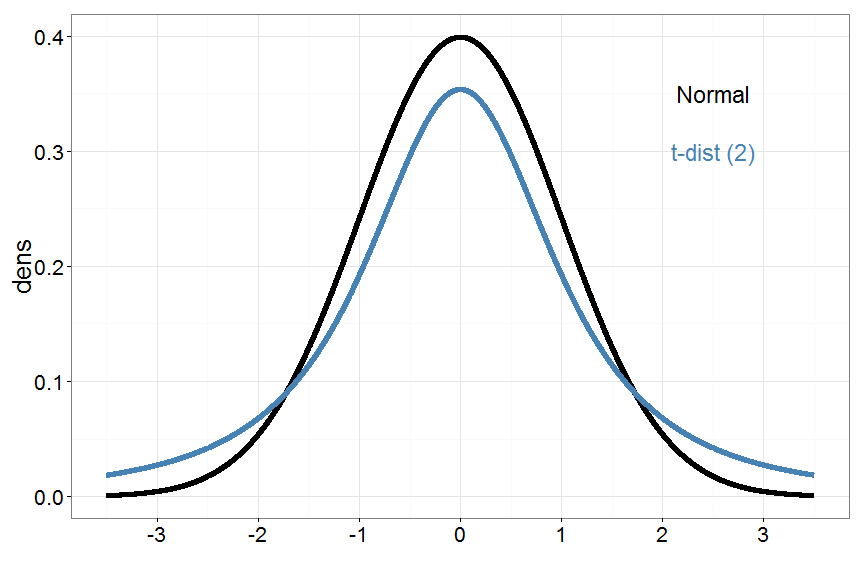
\includegraphics[width=3.5in]{figure/normvst-1.png}
\caption{plot of chunk normvst}
\end{figure}

\section{Comparing t-distribution to normal
distribution.}\label{comparing-t-distribution-to-normal-distribution.-1}

\begin{itemize}
\item
  Formula comparisons:\\Population SD:
  \(\sigma = \sqrt{\frac{\sum(X - \bar{X})^2}{n}}\) z-score:
  \(z_{obs} = \frac{\bar{X} - \mu}{\frac{\sigma}{\sqrt{n}}}\)\\Sample
  SD: \(s = \sqrt{\frac{\sum(X - \bar{X})^2}{n}}\) t-score:
  \(t_{obs} = \frac{\bar{X} - \mu}{\frac{s}{\sqrt{n-1}}}\), \(df = n - 1\)
\item
  As the degrees of freedom increase, the distribution becomes closer to
  a normal distribution (i.e.~the tails have fewer values in them and
  more values fall in the center of the distribution.)
\end{itemize}

\section{Degrees of Freedom}\label{degrees-of-freedom}

\[ \frac{s}{\sqrt{n-1}} \]\\
\begin{itemize}
\item Degrees of freedom refers to the \(n-1\) in the denominator. 
\item Suppose we let 5 people pick any number. The only requirement we make is that the sum of these 5
numbers must equal 0. 
\item In this scenario, the first 4 people can pick
any number they want (are ``free to vary''), while the 5th number is
``fixed'' to ensure our sum of the numbers is 0. 
\item More generally from
the sample standard deviation above, we say that \(n-1\) numbers are
``free to vary''.
\end{itemize}

\section{Confidence Interval for
t-distribution}\label{confidence-interval-for-t-distribution}

\begin{itemize}
\itemsep1pt\parskip0pt\parsep0pt
\item
  To calculate a confidence interval for the population mean when the
  population standard deviation is unknown:\\C\% CI of \(\mu\):
  \(\bar{X} \pm t_{crit} * \frac{s}{\sqrt{n - 1}}\)\\
\item
  Where \(\pm t_{crit}\) are the t-scores such that the proportion (or area) of
  the curve within the t-scores is equal to the confidence level.
\end{itemize}

\section{Example}\label{example-1}

\begin{itemize}
\itemsep1pt\parskip0pt\parsep0pt
\item
  A team statistician for the University of Iowa wants to estimate
  the average number of points the team will score during the season. A
  random sample of 18 games was selected from the past two seasons; the
  average number of points scored was 27.4, and the standard deviation
  was 4.7.

  \begin{itemize}
  \itemsep1pt\parskip0pt\parsep0pt
  \item
    What is the best point estimate of the population mean?\\
  \item
    What is the standard error?
  \item
    What is the 95\% confidence interval?
  \item
    What is the 99\% confidence interval?
  \end{itemize}
\end{itemize}

\section{Big Picture for Inferential
Statistics}\label{big-picture-for-inferential-statistics}

\begin{enumerate}
\def\labelenumi{\arabic{enumi}.}
\itemsep1pt\parskip0pt\parsep0pt
\item
  Establish a Research Hypothesis.
\item
  Choose statistical test to use based on research question and
  data/information you have.
\item
  Make a null and alternative hypothesis, one-tailed or two tailed
  hypotheses.
\item
  Set level of significance (type I/II Error).

  \begin{itemize}
  \itemsep1pt\parskip0pt\parsep0pt
  \item
    Find a critical value.
  \item
    How confident do you want to be?
  \end{itemize}
\item
  Calculate test statistic.

  \begin{itemize}
  \itemsep1pt\parskip0pt\parsep0pt
  \item
    Find a p-value.
  \end{itemize}
\item
  Reach statistical conclusion.
\item
  Make a research conclusion (i.e.~translate statistical conclusion into
  real world terminology).
\end{enumerate}

\section{Research Question and Type of
Test}\label{research-question-and-type-of-test}

\begin{itemize}
\itemsep1pt\parskip0pt\parsep0pt
\item
  What are you interested in knowing?
\item
  What are you trying to discover by doing your research?
\item
  One sample tests analyze a sample's mean versus the population mean.

  \begin{itemize}
  \itemsep1pt\parskip0pt\parsep0pt
  \item
    Use a Z-test when the population standard deviation is known.
  \item
    Use a t-test when the population standard deviation is unknown.
  \end{itemize}
\end{itemize}

\section{Hypotheses}\label{hypotheses}

\begin{itemize}
\itemsep1pt\parskip0pt\parsep0pt
\item
  A hypothesis is a proposed explanation for a problem.
\item
  The hypothesis is the general ``blue-print'' for collecting and
  interpreting data.
\item
  A hypothesis provides direction to the research.

  \begin{itemize}
  \itemsep1pt\parskip0pt\parsep0pt
  \item
    Helps us specify the population, what type of data we need,
    relationship between variables, statistical analyses to use.
  \end{itemize}
\item
  A statistical hypothesis provides a specific relational statement that
  can be statistically tested.
\item
  \textbf{The statistical hypothesis is always stated in terms of
  population parameter} (\(\mu\) for now).
\item
  Can state the hypothesis with words and in notation.
\item
  The type of test being conducted influences how the hypothesis will be
  stated.
\end{itemize}

\section{Types of Hypotheses}\label{types-of-hypotheses}

\begin{itemize}
\itemsep1pt\parskip0pt\parsep0pt
\item
  \textbf{Null Hypthosis} (\(H_{0}\)): statement that there is NO
  relationship, NO impact, or NO difference.
\item
  We assume the null hypothesis is true and test against the null
  hypothesis.

  \begin{itemize}
  \itemsep1pt\parskip0pt\parsep0pt
  \item
    We ultimately make statements about the likelihood the null
    hypothesis is true.
  \end{itemize}
\item
  The conclusions are stated in terms of the null hypothesis:

  \begin{itemize}
  \itemsep1pt\parskip0pt\parsep0pt
  \item
    \emph{Reject the null hypothesis}, which is not agreeing with the
    null hypothesis.
  \item
    \emph{Fail to reject the null hypothesis}, which is a statement of
    agreement with the null hypothesis. We never ``accept'' the null
    hypothesis, just provide evidence that our sample is not different
    from the population.
  \end{itemize}
\end{itemize}

\section{Types of Hypotheses 2}\label{types-of-hypotheses-2}

\begin{itemize}
\itemsep1pt\parskip0pt\parsep0pt
\item
  \textbf{Alternative Hypothesis} (\(H_{1}\) or \(H_{a}\)): statement
  that there IS a relationship among variables or that there is a
  difference between groups.
\item
  For conclusions, \emph{failing to reject the null hypothesis} provides
  evidence in favor of the alternative hypothesis.
\end{itemize}

\section{Hypotheses for one-sample
tests}\label{hypotheses-for-one-sample-tests}

\begin{itemize}
\itemsep1pt\parskip0pt\parsep0pt
\item
  Non-directional (two-tailed) test:\\\(H_{0}: \mu = \mu_{0}\) and
  \(H_{1}: \mu \neq \mu_{0}\)
\item
  Directional (one-tailed) test:\\\(H_{0}: \mu = \mu_{0}\) and
  \(H_{1}: \mu > \mu_{0}\) right tailed\\\(H_{0}: \mu = \mu_{0}\) and
  \(H_{1}: \mu < \mu_{0}\) left tailed
\end{itemize}

where \(\mu_{0}\) is the proposed population mean that is to be tested.

\section{One-tailed vs two-tailed
Hypotheses}\label{one-tailed-vs-two-tailed-hypotheses}

\begin{itemize}
\itemsep1pt\parskip0pt\parsep0pt
\item
  With a two-tailed (non-directional) test, you reject the null
  hypothesis if the sample mean is \textbf{either} significantly greater
  or less than the hypothesized value.
\item
  In a one-tailed (directional) test, the null hypothesis would not be
  rejected unless the observed difference is in the hypothesized
  direction.

  \begin{itemize}
  \itemsep1pt\parskip0pt\parsep0pt
  \item
    The direction of the hypothesis affects which areas within the curve
    result in a rejection of \(H_{0}\). It also influences our choice
    for a critical value.
  \end{itemize}
\end{itemize}

\section{Hypothesis Example 1}\label{hypothesis-example-1}

Question: Is the average price of gas in Iowa City less than the
national average of \$2.30?\\ \(H_{0}:\)\\ \(H_{1}:\)

\section{Hypothesis Example 2}\label{hypothesis-example-2}

Question: Is the average Big 10 college football head coaches salary
greater than the national average of \$1.64 million?\\ \(H_{0}:\)\\
\(H_{1}:\)

\section{Level of Significance}\label{level-of-significance}

\begin{itemize}
\itemsep1pt\parskip0pt\parsep0pt
\item
  \textbf{Level of Significance} (i.e. \(\alpha\)-level) is a
  predetermined level of rejecting the null when it is actually true.
\item
  The level of significance is the area in the tail of direction stated
  in the hypothesis is equal to \(\alpha\).
\item
  Confidence level (make correct conclusion C\% of the time)
  \(C = 1 - \alpha\)
\item
  Common values for \(\alpha\) include: .05, .01, .001.
\item
  The researcher \emph{chooses} how confident he or she wants to be in
  their test. This also determines the chance of error the researcher is
  willing to make.
\end{itemize}

\section{Critical Values}\label{critical-values}

\begin{itemize}
\itemsep1pt\parskip0pt\parsep0pt
\item
  Critical values are the values that separate the distribution into
  regions where the null hypothesis will be rejected or regions where
  the null hypothesis will failed to be rejected.
\item
  The critical values separates the rejection region from the
  non-rejection region.
\item
  Critical values are found using the distribution tables.
\item
  To find a critical value, we need to know the level of significance,
  direction of test, and degrees of freedom (except for z-critical
  values).
\end{itemize}

\section{Rejection region}\label{rejection-region}

\begin{itemize}
\itemsep1pt\parskip0pt\parsep0pt
\item
  The rejection region is the range of values for which the null
  hypothesis is not probable.

  \begin{itemize}
  \itemsep1pt\parskip0pt\parsep0pt
  \item
    It is always in the direction of the alternative hypothesis.
  \item
    The total area of the rejection area equal \(\alpha\).
  \end{itemize}
\item
  If our test statistic is so large that it falls in the rejection
  region, your conclusion is to reject the null hypothesis.
\end{itemize}

\section{Two-tailed Rejection Region}\label{two-tailed-rejection-region}

\begin{itemize}
\itemsep1pt\parskip0pt\parsep0pt
\item
  For a level of significance of \(\alpha = 0.05\), the rejection region
  for a normal distribution would look like:
\end{itemize}

\begin{figure}[H]
\centering
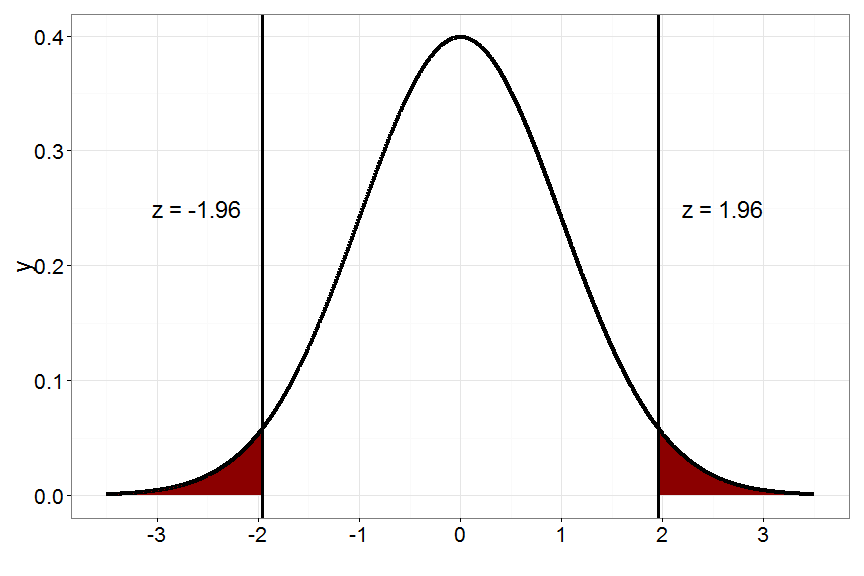
\includegraphics[width=3.5in]{figure/rejectz-1.png}
\caption{plot of chunk rejectz}
\end{figure}

\section{One-tailed Rejection Region (greater
than)}\label{one-tailed-rejection-region-greater-than}

\begin{itemize}
\itemsep1pt\parskip0pt\parsep0pt
\item
  For a level of significance of \(\alpha = 0.05\), the rejection region
  for a normal distribution would look like:
\end{itemize}

\begin{figure}[H]
\centering
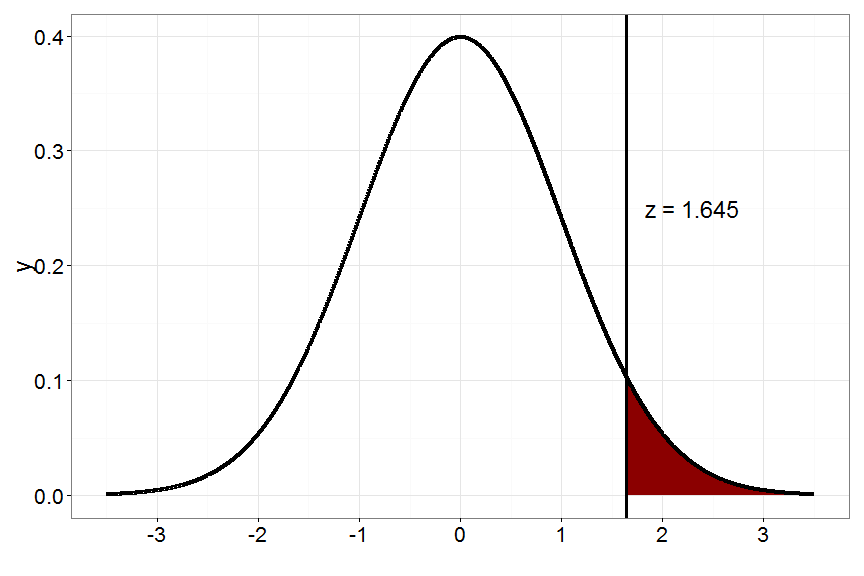
\includegraphics[width=3.5in]{figure/rejectzoneg-1.png}
\caption{plot of chunk rejectzoneg}
\end{figure}

\section{One-tailed Rejection Region (less
than)}\label{one-tailed-rejection-region-less-than}

\begin{itemize}
\itemsep1pt\parskip0pt\parsep0pt
\item
  For a level of significance of \(\alpha = 0.05\), the rejection region
  for a normal distribution would look like:
\end{itemize}

\begin{figure}[H]
\centering
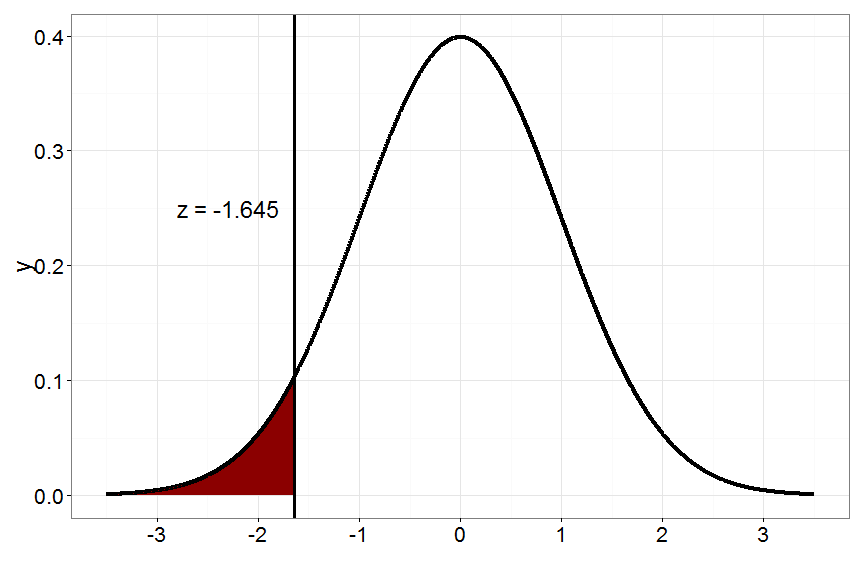
\includegraphics[width=3.5in]{figure/rejectzonel-1.png}
\caption{plot of chunk rejectzonel}
\end{figure}

\section{Critical Value Example}\label{critical-value-example}

\begin{itemize}
\itemsep1pt\parskip0pt\parsep0pt
\item
  Z

  \begin{itemize}
  \itemsep1pt\parskip0pt\parsep0pt
  \item
    What are the critical values for a two-tailed z-test with
    \(\alpha = .05\)?
  \item
    What are the critical values for a left-tailed z-test with
    \(\alpha = .02\)?
  \end{itemize}
\item
  T

  \begin{itemize}
  \itemsep1pt\parskip0pt\parsep0pt
  \item
    What are the critical values for a two-tailed t-test with
    \(\alpha = .05\) and degrees of freedom of 10?
  \item
    What are the critical values for a right-tailed t-test with
    \(\alpha = .05\) and degrees of freedom of 25?
  \end{itemize}
\end{itemize}

\section{Test Statistic}\label{test-statistic}

\begin{itemize}
\itemsep1pt\parskip0pt\parsep0pt
\item
  The type of test determines how the test statistic is calculated.
\item
  In this class we will talk about these tests:

  \begin{itemize}
  \itemsep1pt\parskip0pt\parsep0pt
  \item
    One-sample z-test
  \item
    One-sample t-test
  \item
    Independent t-test
  \item
    Dependent/paired t-test
  \end{itemize}
\end{itemize}

\section{Test Statistic - One Sample
Z-test}\label{test-statistic---one-sample-z-test}

\begin{itemize}
\itemsep1pt\parskip0pt\parsep0pt
\item
  A test for quantitative data.
\item
  Information given (known):

  \begin{itemize}
  \itemsep1pt\parskip0pt\parsep0pt
  \item
    Population mean (\(\mu\))
  \item
    Population standard deviation (\(\sigma\))
  \end{itemize}
\item
  Questions answered:

  \begin{itemize}
  \itemsep1pt\parskip0pt\parsep0pt
  \item
    Did a particular sample come from a given population?
  \item
    Is a sample mean significantly different/less than/greater than the
    population mean?
  \end{itemize}
\end{itemize}

\section{\texorpdfstring{One Sample Z-test:
\(z_{obs}\)}{One Sample Z-test: z\_\{obs\}}}\label{one-sample-z-test-zux5fobs}

\begin{itemize}
\itemsep1pt\parskip0pt\parsep0pt
\item
  Formula:\\\(z_{obs} = \frac{\bar{X} - \mu}{\frac{\sigma}{\sqrt{n}}}\)\\where
  \(\bar{X}\) is the sample mean,\\\(\mu\) is the population mean
  (given),\\\(\sigma\) is the population standard deviation
  (given),\\\(n\) is the sample size.
\end{itemize}

\section{Test Statistic t-test}\label{test-statistic-t-test}

\begin{itemize}
\itemsep1pt\parskip0pt\parsep0pt
\item
  A test for quantitative data.
\item
  Information given (known):

  \begin{itemize}
  \itemsep1pt\parskip0pt\parsep0pt
  \item
    Population mean (\(\mu\))
  \item
    \emph{Sample} standard deviation (\(s\))
  \end{itemize}
\item
  Questions answered:

  \begin{itemize}
  \itemsep1pt\parskip0pt\parsep0pt
  \item
    Did a particular sample come from a given population?
  \item
    Is a sample mean significantly different/less than/greater than the
    population mean?
  \end{itemize}
\end{itemize}

\section{\texorpdfstring{One Sample t-test:
\(t_{obs}\)}{One Sample t-test: t\_\{obs\}}}\label{one-sample-t-test-tux5fobs}

\begin{itemize}
\itemsep1pt\parskip0pt\parsep0pt
\item
  Formula:\\\(t_{obs} = \frac{\bar{X} - \mu}{\frac{s}{\sqrt{n - 1}}}\)\\where
  \(\bar{X}\) is the sample mean,\\\(\mu\) is the population mean (given
  or calculated from sample),\\\(s\) is the sample standard deviation
  (given or calculated from sample),\\\(n\) is the sample size.
\end{itemize}

\section{Statistical Conclusion}\label{statistical-conclusion}

\begin{itemize}
\itemsep1pt\parskip0pt\parsep0pt
\item
  If the test statistic (either \(z_{obs}\) or \(t_{obs}\)) falls in the
  ``rejection region,'' or outside of the critical value(s), the
  conclusion is to \textbf{reject the null hypothesis}.

  \begin{itemize}
  \itemsep1pt\parskip0pt\parsep0pt
  \item
    More formally, we state that the results are ``statistically
    significant'' with a certain confidence level.
  \end{itemize}
\item
  If the observed test statistic (either \(z_{obs}\) or \(t_{obs}\))
  does not fall in the ``rejection region,'' or inside of the critical
  value(s), the conclusion is to \textbf{fail to reject the null
  hypothesis}.
\end{itemize}

\section{Research Conclusion}\label{research-conclusion}

\begin{itemize}
\itemsep1pt\parskip0pt\parsep0pt
\item
  The statistical conclusion can also be stated in terms of words.
\item
  If we \textbf{reject the null hypothesis}, we can state that the
  sample mean differs, is greater than, or less than the population
  mean.

  \begin{itemize}
  \itemsep1pt\parskip0pt\parsep0pt
  \item
    The direction we can conclude stems back to the direction of our
    research hypotheses.
  \end{itemize}
\item
  If we \textbf{fail to reject the null hypothesis}, we state that the
  sample mean does not differ, is not greater than, or is less than the
  population mean.
\end{itemize}

\section{p-value}\label{p-value}

\begin{itemize}
\itemsep1pt\parskip0pt\parsep0pt
\item
  The \textbf{p-value} is the probability of obtaining a result at least
  as extreme as the one that was actually observed, given that the null
  hypothesis is true.
\item
  This probability corresponds to the area greater than the observed
  test-statistic, either \(z_{obs}\) or \(t_{obs}\).
\item
  When the conclusion is to \textbf{reject the null hypothesis} it is
  known that \(p < \alpha\).
\item
  When the conclusion is to \textbf{fail to reject the null hypothesis}
  it is known that \(p > \alpha\).
\end{itemize}

\section{Visualizing p-value}\label{visualizing-p-value}

\begin{itemize}
\itemsep1pt\parskip0pt\parsep0pt
\item
  Suppose we have a z-obs value of 2.3 with a one-tailed greater than
  hypothesis.
\end{itemize}

\begin{figure}[H]
\centering
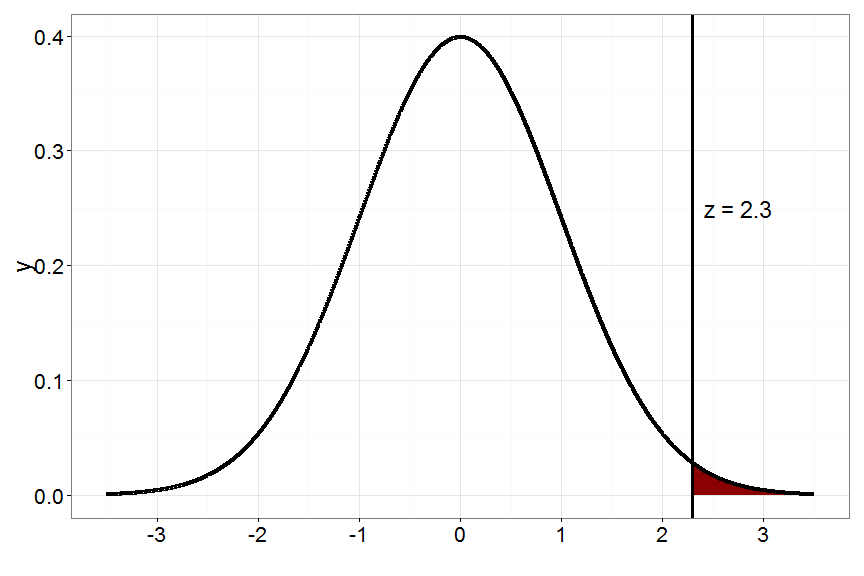
\includegraphics[width=3.5in]{figure/pvaluegreater-1.png}
\caption{plot of chunk pvaluegreater}
\end{figure}

\section{Visualizing p-value 2}\label{visualizing-p-value-2}

\begin{itemize}
\itemsep1pt\parskip0pt\parsep0pt
\item
  Suppose we have a z-obs value of 2.3 with a two-tailed hypothesis.
\end{itemize}

\begin{figure}[H]
\centering
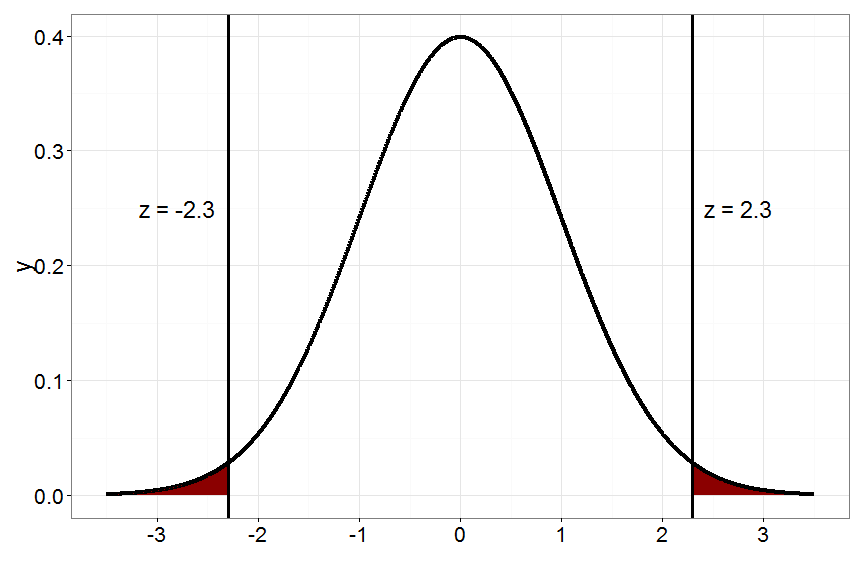
\includegraphics[width=3.5in]{figure/pvalueless-1.png}
\caption{plot of chunk pvalueless}
\end{figure}

\section{Example}\label{example-3}

The average individual works out an average of 3.75 hours per week (45
minutes, 5 days a week), with a standard deviation of 1 hour. Suppose we
collect a sample of 159 participants and the sample mean was 4.87 hours
of exercise per week. Is our sample mean significantly greater than the
national population at \(\alpha = .05\)?



\section{Example 2}\label{example-2-1}

The average height for US females 20 years and older is about 64 inches
with a standard deviation about 4 inches. A sample of 28 players from
the UI women's soccer team has an average height of 66.6 inches. How
likely is it that the UI women's soccer team is significantly taller
than the adult female population with an \(\alpha = .05\)?



\section{Example 3}\label{example-3-1}

Suppose you conduct an experiment to see if a given therapy works to
reduce test anxiety in a sample of college students. A standard measure
of test anxiety is known to produce a population mean (\(\mu\)) of 20.
With your sample of 61 students, the mean is 18 and the standard
deviation is 9. Use an \(\alpha = .05\).


\end{document}
